% Options for packages loaded elsewhere
\PassOptionsToPackage{unicode}{hyperref}
\PassOptionsToPackage{hyphens}{url}
%
\documentclass[
  12,
  a4paper,
]{report}
\usepackage{amsmath,amssymb}
\usepackage{lmodern}
\usepackage{setspace}
\usepackage{iftex}
\ifPDFTeX
  \usepackage[T1]{fontenc}
  \usepackage[utf8]{inputenc}
  \usepackage{textcomp} % provide euro and other symbols
\else % if luatex or xetex
  \usepackage{unicode-math}
  \defaultfontfeatures{Scale=MatchLowercase}
  \defaultfontfeatures[\rmfamily]{Ligatures=TeX,Scale=1}
  \setmainfont[]{Times}
\fi
% Use upquote if available, for straight quotes in verbatim environments
\IfFileExists{upquote.sty}{\usepackage{upquote}}{}
\IfFileExists{microtype.sty}{% use microtype if available
  \usepackage[]{microtype}
  \UseMicrotypeSet[protrusion]{basicmath} % disable protrusion for tt fonts
}{}
\makeatletter
\@ifundefined{KOMAClassName}{% if non-KOMA class
  \IfFileExists{parskip.sty}{%
    \usepackage{parskip}
  }{% else
    \setlength{\parindent}{0pt}
    \setlength{\parskip}{6pt plus 2pt minus 1pt}}
}{% if KOMA class
  \KOMAoptions{parskip=half}}
\makeatother
\usepackage{xcolor}
\IfFileExists{xurl.sty}{\usepackage{xurl}}{} % add URL line breaks if available
\IfFileExists{bookmark.sty}{\usepackage{bookmark}}{\usepackage{hyperref}}
\hypersetup{
  pdflang={fr},
  hidelinks,
  pdfcreator={LaTeX via pandoc}}
\urlstyle{same} % disable monospaced font for URLs
\usepackage[margin=2.5cm]{geometry}
\usepackage{graphicx}
\makeatletter
\def\maxwidth{\ifdim\Gin@nat@width>\linewidth\linewidth\else\Gin@nat@width\fi}
\def\maxheight{\ifdim\Gin@nat@height>\textheight\textheight\else\Gin@nat@height\fi}
\makeatother
% Scale images if necessary, so that they will not overflow the page
% margins by default, and it is still possible to overwrite the defaults
% using explicit options in \includegraphics[width, height, ...]{}
\setkeys{Gin}{width=\maxwidth,height=\maxheight,keepaspectratio}
% Set default figure placement to htbp
\makeatletter
\def\fps@figure{htbp}
\makeatother
\setlength{\emergencystretch}{3em} % prevent overfull lines
\providecommand{\tightlist}{%
  \setlength{\itemsep}{0pt}\setlength{\parskip}{0pt}}
\setcounter{secnumdepth}{5}
\newlength{\cslhangindent}
\setlength{\cslhangindent}{1.5em}
\newlength{\csllabelwidth}
\setlength{\csllabelwidth}{3em}
\newlength{\cslentryspacingunit} % times entry-spacing
\setlength{\cslentryspacingunit}{\parskip}
\newenvironment{CSLReferences}[2] % #1 hanging-ident, #2 entry spacing
 {% don't indent paragraphs
  \setlength{\parindent}{0pt}
  % turn on hanging indent if param 1 is 1
  \ifodd #1
  \let\oldpar\par
  \def\par{\hangindent=\cslhangindent\oldpar}
  \fi
  % set entry spacing
  \setlength{\parskip}{#2\cslentryspacingunit}
 }%
 {}
\usepackage{calc}
\newcommand{\CSLBlock}[1]{#1\hfill\break}
\newcommand{\CSLLeftMargin}[1]{\parbox[t]{\csllabelwidth}{#1}}
\newcommand{\CSLRightInline}[1]{\parbox[t]{\linewidth - \csllabelwidth}{#1}\break}
\newcommand{\CSLIndent}[1]{\hspace{\cslhangindent}#1}
\ifLuaTeX
\usepackage[bidi=basic]{babel}
\else
\usepackage[bidi=default]{babel}
\fi
\babelprovide[main,import]{french}
% get rid of language-specific shorthands (see #6817):
\let\LanguageShortHands\languageshorthands
\def\languageshorthands#1{}
\usepackage{ragged2e} % alignement
\usepackage{setspace} % espace entre les lignes

\usepackage[french]{babel}

% pour les titres de tables et figures
\usepackage[normal,labelfont=bf]{caption}
\usepackage{subcaption}
\captionsetup{format=hang,font=small}
\captionsetup[table]{name=Table}
\captionsetup[figure]{name=Figure}

% pour s'assurer que les notes de bas de page reste bien en bas
\usepackage[bottom]{footmisc}

% pour les encadrés
\usepackage{mdframed}


% pour la police
\usepackage[utf8]{inputenc}
\usepackage[T1]{fontenc}


% pour table des matières
\usepackage{chngcntr}
\counterwithin{figure}{section}
\counterwithin{table}{section}


\usepackage[toc,title,page]{appendix}


\usepackage{amsthm}
\newtheorem{hyp}{Hypothèse}

% Pour ajouter le titre de chapitre dans lequel on est en haut de la page
\usepackage{fancyhdr} 
\pagestyle{fancy}
\fancyhead[LE,RO]{\thechapter}
\ifLuaTeX
  \usepackage{selnolig}  % disable illegal ligatures
\fi

\author{}
\date{\vspace{-2.5em}}

\begin{document}

\setstretch{1.5}
\begin{titlepage}

\par
\raisebox{-.5\height}{
\includegraphics[width=3cm]{logos/Logo_EHESS.jpg}}
\hfill
\raisebox{-.5\height}{
\includegraphics[width=5.5cm]{logos/logo_ens.png}}
\par


\vspace{1cm}
\begin{center}

\normalsize{\textit{Master Sciences Sociales - Parcours Quantifier en Sciences Sociales}}

2021-2022

\vspace{5mm}

\textsc{Mémoire de recherche}

\vfill 

{\LARGE\bfseries Entre famille et institution :\par}

{\Large le parcours de placement en Maison d'enfant à caractère social\par}

\vfill

{\large\itshape Soutenu par}

{\large Élodie Lemaire}

\vspace{5mm}

\textit{Session}

Juin 2022

\vspace{5mm}

\textit{Sous les directions de}

Isabelle Frechon, Ined

\textit{et}

Marie Plessz, Inrae


\vspace{5mm}

\textit{Rapporteur}

Jérôme Deauvieau, Cnrs

\end{center}
\end{titlepage}
\newpage

\pagenumbering{roman}

\phantomsection
\addcontentsline{toc}{section}{Remerciements}
\section*{Remerciements}

Je tiens à remercier

\vspace{.5cm}

\newpage

\newpage
\begin{spacing}{1}
\phantomsection
\addcontentsline{toc}{section}{Table des matières}

\tableofcontents
\listoftables
\listoffigures

\end{spacing}

\newpage
\pagenumbering{arabic}
\setlength{\parskip}{1em}

\newpage

\hypertarget{placer-un-enfant-uxe0-la-protection-de-lenfance-enjeux-et-fonctionnement}{%
\chapter{Placer un enfant à la Protection de l'enfance : enjeux et
fonctionnement}\label{placer-un-enfant-uxe0-la-protection-de-lenfance-enjeux-et-fonctionnement}}

\emph{Revenir sur nécessité de présenter le fonctionnement de la
Protection de l'enfance qui est assez complexe en France et hérité
d'évolutions sur un temps long.} \emph{Une évolution qui a eu un effet
sur la production de données sur le sujet.} \emph{Et qui donne lieu à
certains types d'établissements qui sont au cœur de ses évolutions et de
l'innovation.}

\hypertarget{la-protection-de-lenfance-en-france-duxe9veloppement-et-fonctionnement}{%
\section{La Protection de l'enfance en France : développement et
fonctionnement}\label{la-protection-de-lenfance-en-france-duxe9veloppement-et-fonctionnement}}

\hypertarget{quest-ce-que-la-protection-de-lenfance}{%
\subsection{Qu'est-ce que la Protection de l'enfance
?}\label{quest-ce-que-la-protection-de-lenfance}}

~~~~~~\emph{La Protection de l'enfance, fonctionnement général}

~~En France, la Protection de l'enfance s'organise depuis la fin de la
Seconde Guerre mondiale en deux branches qui protègent parfois les mêmes
enfants : le judiciaire et l'administratif. La protection judiciaire
s'occupe de deux catégories d'enfants : les enfants délinquants et les
enfants en danger mineurs ou jeunes majeurs. La protection
administrative, prise en charge par l'Aide sociale à l'enfance, s'occupe
des enfants mineurs ou majeurs de moins de 21 ans en risque de danger ou
en danger.

Figure -- Schéma de l'organisation de la Protection de l'enfance en
France

\begin{center}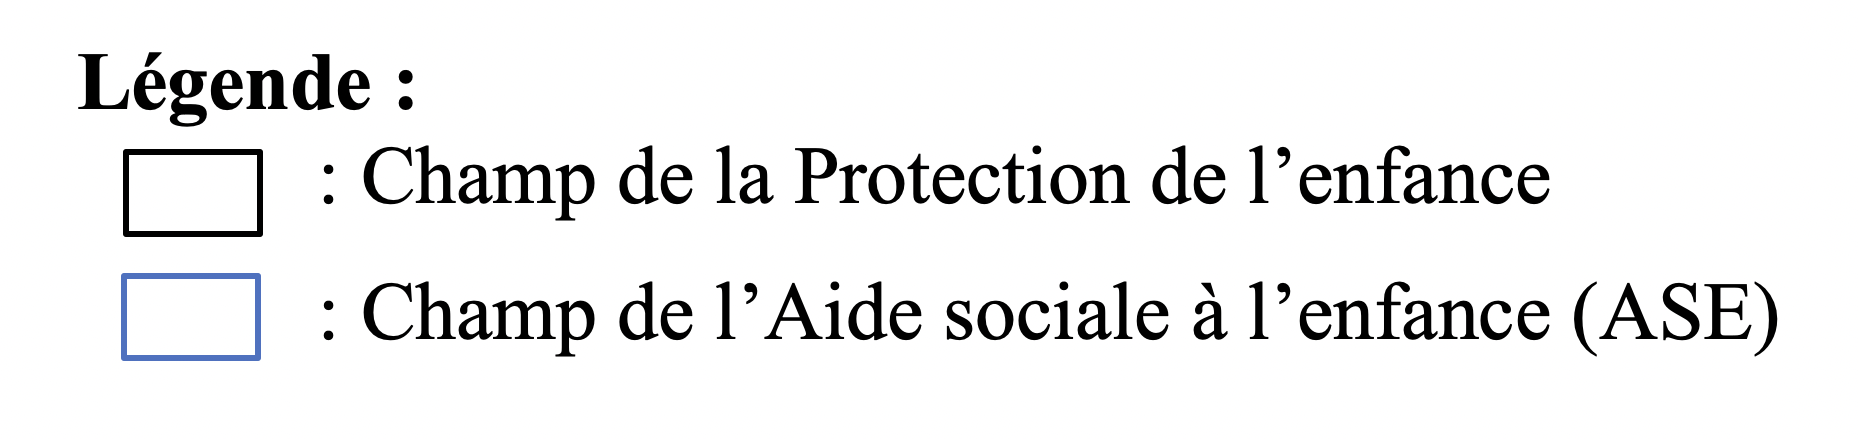
\includegraphics[width=0.4\linewidth]{Figure/SCleg} \end{center}

\begin{center}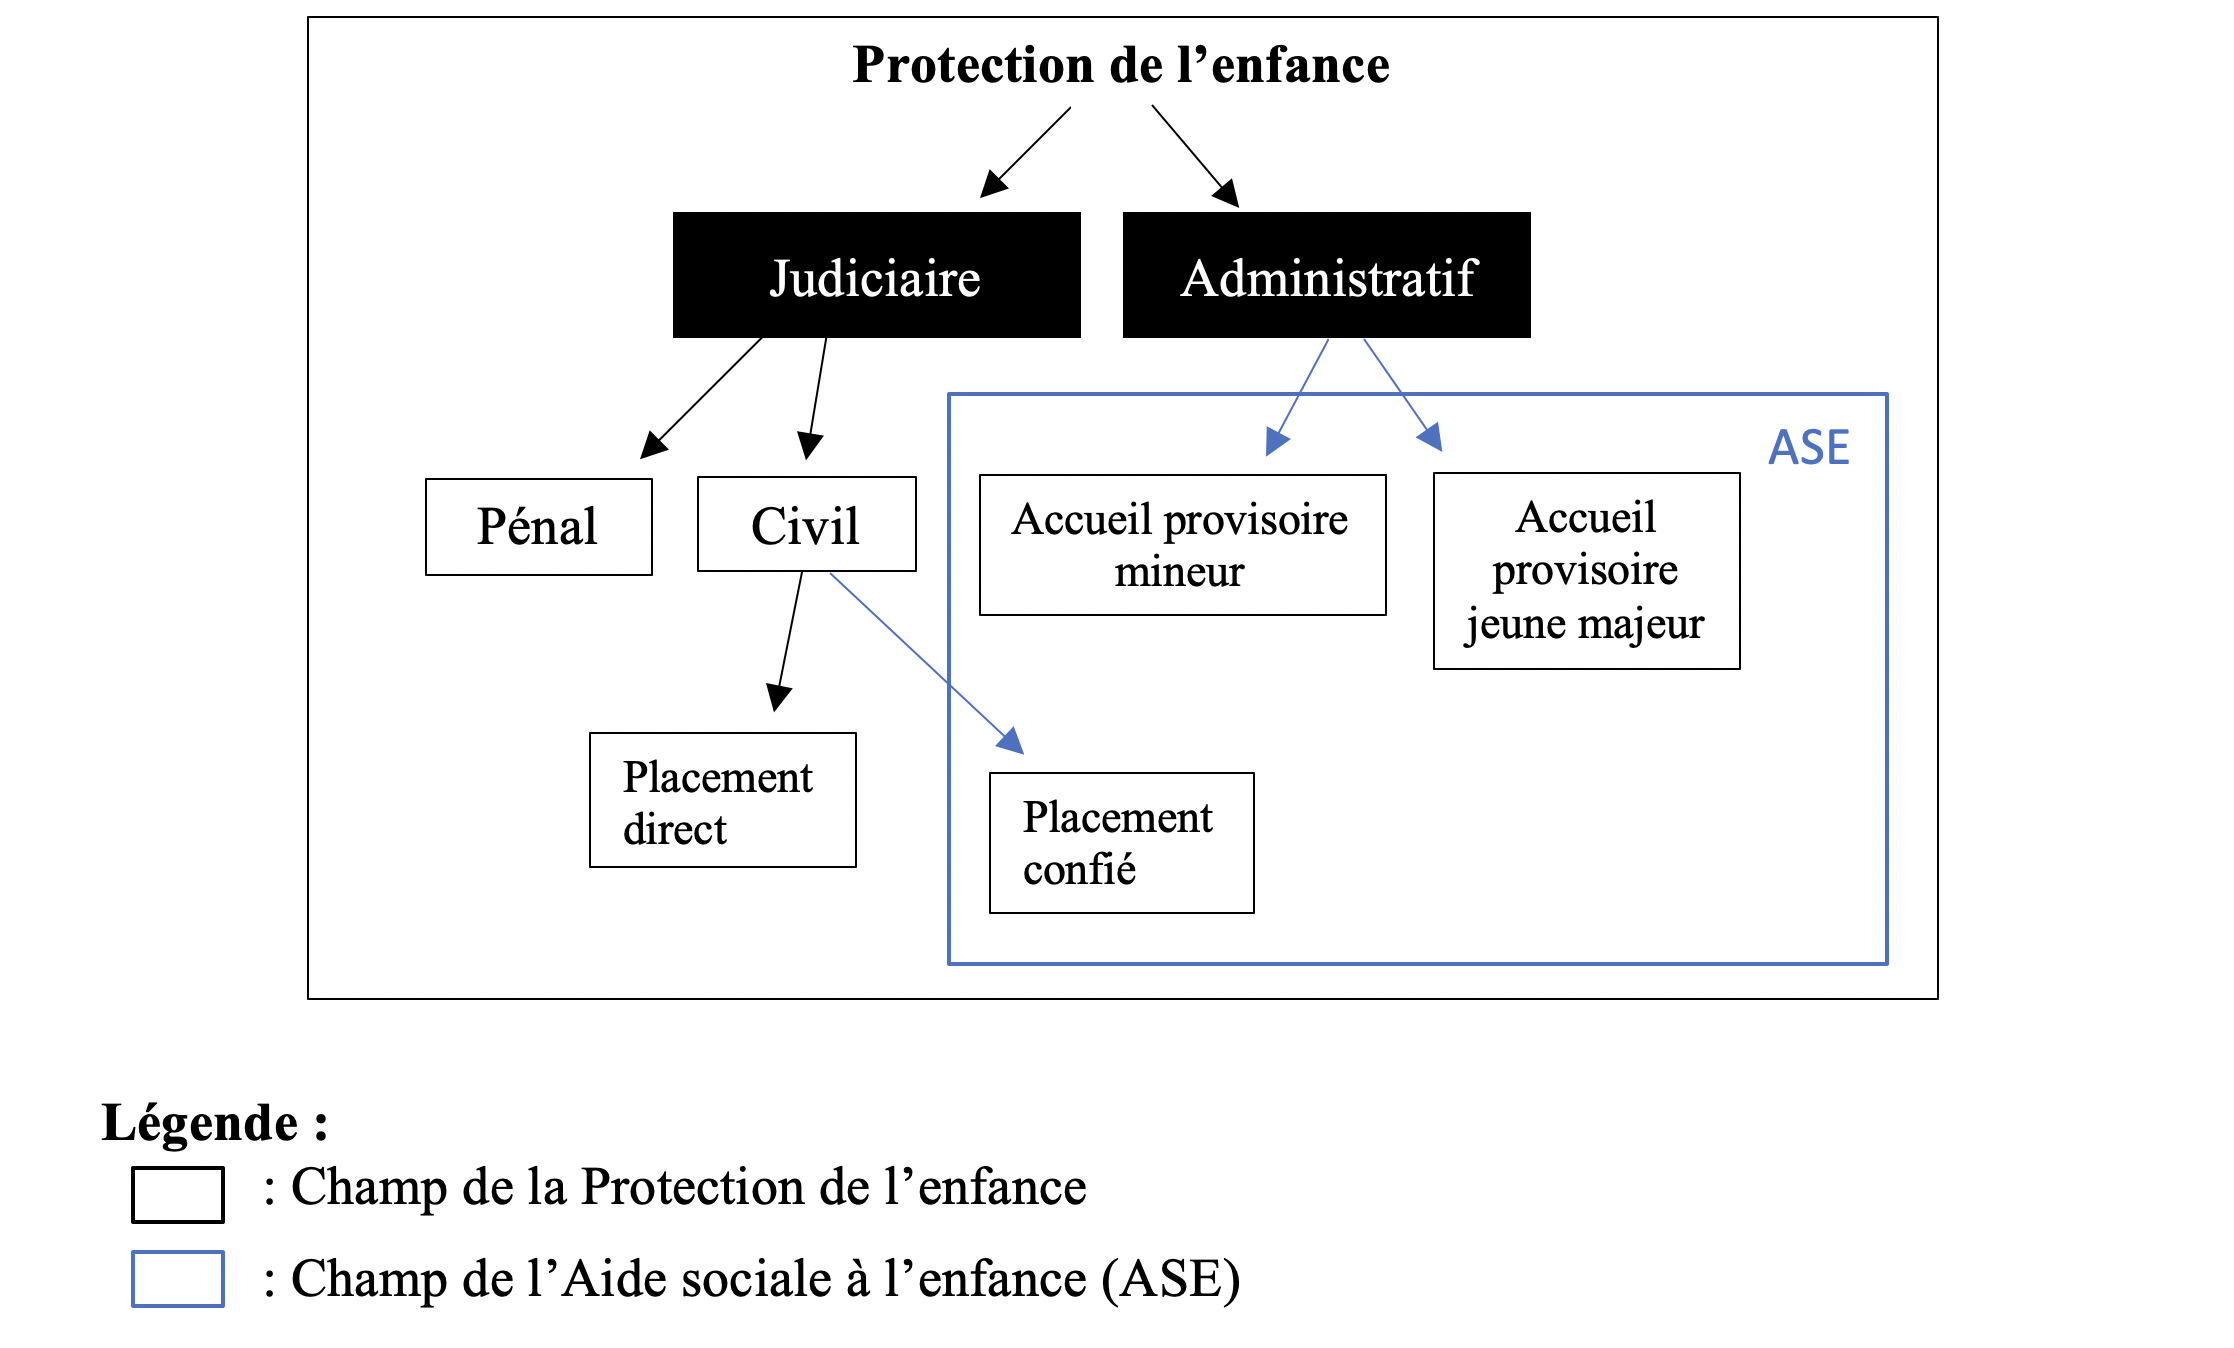
\includegraphics[width=0.6\linewidth]{Figure/SC1} \end{center}

Si on replace la Protection de l'enfance dans le paysage de l'aide
sociale en France, elle entre dans le cadre des systèmes de solidarité
et non dans celui de prévoyance. En effet, les systèmes de prévoyance
sont financés par les cotisations et donc ouverts qu'à ceux qui y
cotisent. Les systèmes de solidarité quant à eux s'applique à des
personnes qui n'ont pas cotisé. Il s'agit de ce fait d'une aide
subsidiaire, puisqu'elle n'intervient qu'en cas de défaillance ou
déficience de la famille, puis du droit commun . La Protection de
l'enfance par sa fonction remplit un droit fondamental stipulé par
l'article 11 du préambule de la Constitution de 1946 garantissant « à
tous, notamment à l'enfant, à la mère et aux vieux travailleurs la
protection de la santé, la sécurité matérielle, le repos et les loisirs.
».

~~\emph{La protection judiciaire}

Nous le disions, la protection judiciaire s'occupe à la fois des enfants
délinquants et des enfants en danger mineurs ou jeunes majeurs. Dans les
deux cas, c'est le Tribunal pour enfants représenté par le Juge pour
enfants qui décide de la mesure éducative qui sera prise.

Pour les mineurs délinquants, la mesure prise peut être un placement
chez ses parents ou son tuteur, tout comme un placement sous liberté
surveillée (le mineur sera suivi par un éducateur dépendant directement
du tribunal) et/ou un placement dans une institution ou un établissement
public ou privé d'éducation ou de formation professionnelle habilité. La
mesure ne peut excéder l'âge de 18 ans.

Dans le cas des enfants en dangers mineurs ou jeunes majeurs, le juge
des enfants peut décider de mesures éducatives. En la matière, c'est
l'ordonnance de 1958 relative à la protection de l'enfance et de
l'adolescence en danger qui spécifie le champ et l'objectif de l'action
du juge des enfants en indiquant que le juge ne travaille désormais
aussi dans le domaine du civil et n'est plus restreint au pénal . Ainsi,
ce dernier doit vérifier qu'il s'agit bien d'un cas d'enfant en danger
ou en risque de danger. Une fois cette première étape remplie, il
oriente l'enfant soit en protection administrative ou il détermine
l'absence de danger et se retire du dossier. N'existant pas de
définition claire d'enfant en situation de danger, ce point est laissé à
l'appréciation personnelle du juge des enfants. Dans le cas d'un choix
d'action de la part du juge, ce dernier peut choisir de la faire
appliquer avec ou sans l'accord des parents ou des tuteurs légaux. Il
doit néanmoins par la loi chercher le plus possible l'adhésion de la
famille. Les enfants de cette catégorie peuvent être pris en charge
jusqu'à l'âge de 21 ans.

~~~\emph{La protection administrative}

Concernant, la branche administrative de la Protection de l'enfance,
cette dernière est gérée par l'Aide sociale à l'enfance (ASE),
anciennement appelée assistance publique. Elle a autant un rôle
préventif que protecteur . Pour appliquer une mesure, elle doit
impérativement obtenir le consentement des parents ou du/des tuteurs
légaux.

Deux ensembles de moyens d'actions sont menés par l'ASE : les actions
collectives et les prestations individuelles. Les actions collectives
ont pour objectif la promotion sociale et l'insertion des enfants et des
familles. Les prestations individuelles sont soit des aides à domicile,
soit l'accueil de l'enfant dans des structures de l'ASE à la demande des
parents ou suite à une décision judiciaire .

L'ASE a connu une suite de changements législatifs importants également
depuis la fin de la Seconde Guerre mondiale, mais particulièrement lors
de la décentralisation au début des années 1980. L'ASE est en effet un
service départemental depuis la loi du 22 juillet 1983. L'état laisse
ainsi à la charge de chaque département d'organiser ce service d'aide
sociale obligatoire. L'objectif de l'ASE est d'apporter un soutien
matériel, éducatif et psychologique aux mineurs et jeunes majeurs, à
leur famille ou à leurs responsables légaux qui seraient confrontés à
des difficultés mettant ou risquant de mettre en danger la sécurité, la
santé, la moralité, l'éducation, le développement physique affectif,
intellectuel et social, des mineurs ou jeunes majeurs. Le public
concerné est aussi vaste que la mission de l'ASE. Elle accueille ainsi
les mineurs émancipés, les majeurs de moins de 21 ans, les mineurs
isolés, les femmes seules avec enfants de moins de 3 ans.

~~\emph{Des critiques et des évolutions}

Les critiques envers la Protection de l'enfance sont depuis longtemps
virulentes, particulièrement envers le fonctionnement de l'ASE. Elles
dépeignent un service d'accueil violent, qui agirait plus à l'encontre
des familles qu'en leur faveur . Rapidement, face à ces critiques, les
politiques publiques ont évolué. D'abord avec la loi de 2002, qui revoit
le cadre d'intervention en réaffirmant les droits des usagers, qu'ils
s'agissent de l'enfant (mineur ou majeur) ou des familles et en assurant
leur participation dans la vie des établissements. La réforme de la
protection de l'enfance de mars 2007 confirme quant à elle l'ensemble
des dernières évolutions législatives et institue les Conseils Généraux
comme en charge du plan départemental. Elle pose aussi trois axes
prioritaires pour l'avenir de la Protection de l'enfance : renforcer les
actions de prévention sur les territoires, organiser le recueil des
signalements des situations de danger sur les départements, et
diversifier les modes de prises en charge pour les adapter aux besoins
de chaque enfant en danger ou en risque de danger. Cette loi sera enfin
complétée par celle du 14 mars 2016 qui inscrit notamment dans les
missions de l'ASE de veiller à la stabilité du parcours de l'enfant.
Outre des réformes sur certains points légaux de l'adoption, cette loi
réécrit aussi l'article du code de l'action sociale et des familles
relatif au projet pour l'enfant (PPE) afin qu'il serve l'intérêt
supérieur de l'enfant. Enfin, autre développement majeur porté par la
loi de 2016, est l'ajout aux missions des observatoires départementaux
de la protection de l'enfance d'une mission pour la formation continue
des professionnels de la PE .

\hypertarget{un-duxe9veloppement-en-lien-avec-luxe9volution-de-la-notion-de-famille-et-de-la-perception-de-lenfance}{%
\subsection{Un développement en lien avec l'évolution de la notion de
famille et de la perception de
l'enfance}\label{un-duxe9veloppement-en-lien-avec-luxe9volution-de-la-notion-de-famille-et-de-la-perception-de-lenfance}}

~~~~\emph{Les évolutions de la famille contemporaine et l'intervention
croissante de l'état}

Pour comprendre l'institution qu'est la Protection de l'enfance et son
champ professionnel, il faut saisir l'arrière-fond des connaissances,
des savoirs, des normes sociales, voire des prescriptions, en matière de
famille et d'enfance, puisque cet arrière-fond sous-tend leur action.
Nous nous concentrerons d'abord sur la famille avant de porter notre
regard sur l'enfance.

Bien qu'il serait pertinent d'effectuer un retour historique, déjà
mainte fois réalisé, sur la famille au travers des sociétés médiévales
et modernes, tant il éclaire la forme actuelle de la famille
contemporaine, nous nous attarderons sur les évolutions récentes de
l'institution familiale depuis le début du XXe siècle . En effet, durant
ce siècle, la famille a connu des changements majeurs qui peuvent être
résumés dans des facteurs démographiques : la baisse du taux de
mortalité infantile et du taux de natalité, la diffusion des méthodes
modernes de contraception, la légalisation de l'avortement, la réduction
de la taille de la famille. Parallèlement à ces éléments, l'émergence de
l'état-providence a poussé à une plus forte implication de l'état dans
les sujets sociétaux . Ainsi, en France, dans l'exemple des politiques
concernant la jeunesse, ces dernières suivent une logique «
sociale-démocrate » qui tendent à atténuer la dépendance du jeune à sa
famille avec des aides directes de l'état (Frechon, Breugnot et Marquet,
2017 ; Van de Velde, 2012). Un cadre législatif et de nombreuses
réformes ont été mises en place et ont fait évoluer la forme et l'action
de la Protection de l'Enfance, et ce, particulièrement depuis la fin de
la Seconde Guerre mondiale.

Ces évolutions aboutissent à la mise en place de la famille
contemporaine, pour reprendre les réflexions de François de Singly. Ce
dernier démontre le phénomène d'intervention croissante de l'état dans
la famille qui se fait en parallèle avec une privatisation de cette
dernière . C'est dans ce double mouvement que la Protection de l'enfance
s'inscrit en ce faisant un outil de l'intervention étatique au sein de
l'institution familiale. F. de Singly reprend ainsi les suites de la
sociologie de la famille développée par émile Durkheim qui la percevait
déjà comme à la fois privée et publique, privée car il constatait son
autonomisation vis-vis des voisins, publique parce que sa dépendance à
l'état ne cessait de croître . Pour F. de Singly, plus qu'un rôle
d'aide, l'état encadre, voire étend son contrôle sur les familles, il se
fait ainsi le régulateur des relations familiales. Ce contrôle croissant
de la parentalité se fait en parallèle de nombreuses réformes sociales
qui garantissent l'autonomisation de l'homme et de la femme en tant que
conjoints .

On peut ainsi s'interroger sur les effets que produisent cette
intervention croissante de l'état dans une perspective critique. Si ces
évolutions peuvent s'apparenter à un développement positif des libertés
individuelles et du respect des droits de l'Homme avec une protection
légale renforcée des enfants, il existe un versant négatif à cette
intervention. En effet, comme Franz Schultheis l'a souligné, elle
augmenterait les risques socioéconomiques pour les familles en
facilitant la séparation conjugale. Ce risque selon lui dépend du sexe,
de la situation familiale ou encore du statut socioéconomique. Il
s'appuie sur l'exemple des mères célibataires qui font face à de lourdes
difficultés économiques. Ce risque rejaillit sur l'enfant et nécessite
pour l'équilibrer une intervention de l'état . Ici, de nouveau, la
Protection de l'enfance tendrait à pallier ce déséquilibre.

Outre ces points, la société chercherait dès lors à responsabiliser
d'autant plus les parents vis-à-vis de leur·s enfant·s. En effet, en
contrepartie d'un gain de liberté individuelle par une plus grande
facilité de se séparer de son.sa conjoint·e, les deux parents doivent
assurer une continuité parentale auprès de leur·s enfant·s. C'est ce que
souligne particulièrement Irène Thery, pour qui dès lors le bien le plus
précieux de la famille est l'enfant qui devient le socle familial .
Ainsi, les attentes envers l'éducation des enfants augmentent,
justifiant d'autant plus une intervention de la Protection de l'enfance
afin d'assurer une égalité de traitement dans les cas où ces attentes ne
seraient pas remplies.

Du fait de ces évolutions sociétales, le droit a dès lors poussé les
états-providence à agir en matière de protection de l'enfant. La
Convention internationale de l'enfant de 1989 (CIDE) , pour ne citer
qu'elle, parachève un ensemble de textes internationaux qui visent à
garantir les droits en tant que citoyens de l'enfant. Ceci s'explique
par une notion mise en avant par la CIDE de 1989 ratifié par la France
en 1990 qui est celle de l'« intérêt de l'enfant ». Dans le droit
français, cette notion apparaît déjà avec la loi de 1904 portant sur
l'organisation de l'Assistance publique, future Aide sociale à
l'enfance. Ce principe est devenu rapidement un leitmotiv des politiques
publiques. Il apparaît dans les textes de loi et fonde plusieurs de ses
principes d'action et définit les objectifs de prise en charge de
l'enfant.

~~\emph{Les représentations de l'enfance et leurs effets sur les
pratiques professionnelles}

L'ensemble de ces réflexions nous amène à nous concentrer plus
particulièrement sur l'enfant et les représentations de l'enfance. Ces
dernières changent et évoluent d'une culture à une autre. La dimension
historique dans le cas français le met clairement en évidence ,
notamment dans l'évolution qu'a connu l'âge du passage à la majorité et
donc de la fin du statut d'enfant. L'enfance est ainsi une catégorie
sociale, qui par rapport aux autres catégories sociales a la
particularité d'être vécue par tout le monde une fois dans leur vie.
Pour aller plus loin dans cette définition de l'enfance, on peut
reprendre les réflexions de Virginie Vinel et Francesca Zaltron, pour
qui l'enfant est un individu qui appartient à une strate sociale
relative à la société et à une époque donnée .

Ce sont donc les adultes qui fondent les représentations de l'enfance et
créé les contours de cette catégorie. Il est intéressant de noter ici,
que depuis la fin du XIXe siècle et durant tout le XXe siècle jusqu'à
nos jours, l'enfant est défini aux yeux de la société par un ensemble de
savoirs psychologiques et médicaux qui dressent des stades de
développement aboutissant à l'adulte, pour reprendre la réflexion de
André Turmel (Turmel, 2013). Ces derniers régularisent et standardisent
les phases physiques et psychologiques de l'enfant. Ils permettent aussi
de définir les besoins vitaux tant en termes physiques qu'émotionnels de
l'enfant en fonction de son âge, des besoins auxquels la famille se doit
de répondre, et à défaut d'elle, auquel l'état doit suppléer. Ce sont
sur ces connaissances qui sont transmises dans le cadre de leur
formation que les professionnels encadrant les mineurs s'appuient et qui
définit leur mode d'action.

Ces évolutions de la perception de l'enfance ont été étudiées par les
sociologues notamment avec les childhood studies dans lesquelles deux
visions s'affrontent : soit observer les enfants comme des adultes en
formation, soit étudier les enfants en tant qu'être présents, en lien
avec la notion d'agency . Il est intéressant de voir dès lors des études
cherchant à souligner l'effet des différents regards portés sur les
enfants dans la recherche, les institutions, les sociétés et comment ces
différents regards se diffusent et questionnent les acteurs des champs
qui encadrent les mineurs . En effet, le travail des professionnels du
secteur de la protection de l'enfance témoigne de l'évolution de ces
visions de la société. En effet, pour reprendre les mots de Jérôme
Delfortie : « L'édifice Protection de l'Enfance a évolué au gré des
différentes lectures de l'enfance par le prisme social. » . Les
relations entre adultes et enfants ont du fait de ces savoirs sur
l'enfance évolué, que cela soit dans le champ familial ou professionnel.
L'état a augmenté aussi son intervention, ce qui a conduit à
judiciariser les rapports avec enfant, pour reprendre les termes de
Alain Renaut. Un point qui a eu pour effet sa libération de l'autorité
traditionnelle . C'est cette libération qui a court depuis le XIXe
siècle et est même datée par certains à la loi du 24 juillet 1889 où
l'état instaure la déchéance des droits de la puissance paternelle, qui
rend possible l'intervention de la Protection de l'Enfance en la
matière. En effet, l'état devient dès lors le protecteur des enfants en
situation de danger ou risque de danger .

\hypertarget{lorganisation-concruxe8te-du-placement}{%
\subsection{L'organisation concrète du
placement}\label{lorganisation-concruxe8te-du-placement}}

~~\emph{Parcours type en Protection de l'enfance}

Jusqu'à présent nous avons vu l'organisation globale de la Protection de
l'enfance, les types d'enfants dont elle s'occupait et les évolutions de
la société dans la perception de l'enfance et de la famille qui explique
son mode d'action. Dans tout cela, le parcours en soi de placement n'a
pas été abordé. Ce dernier suit un déroulement typique qui va du
signalement et de l'évaluation de la situation à sa réévaluation avant
la sortie de placement ou la mise en place d'une nouvelle mesure.

Figure -- Schéma du parcours type de placement en Protection de
l'enfance

\begin{center}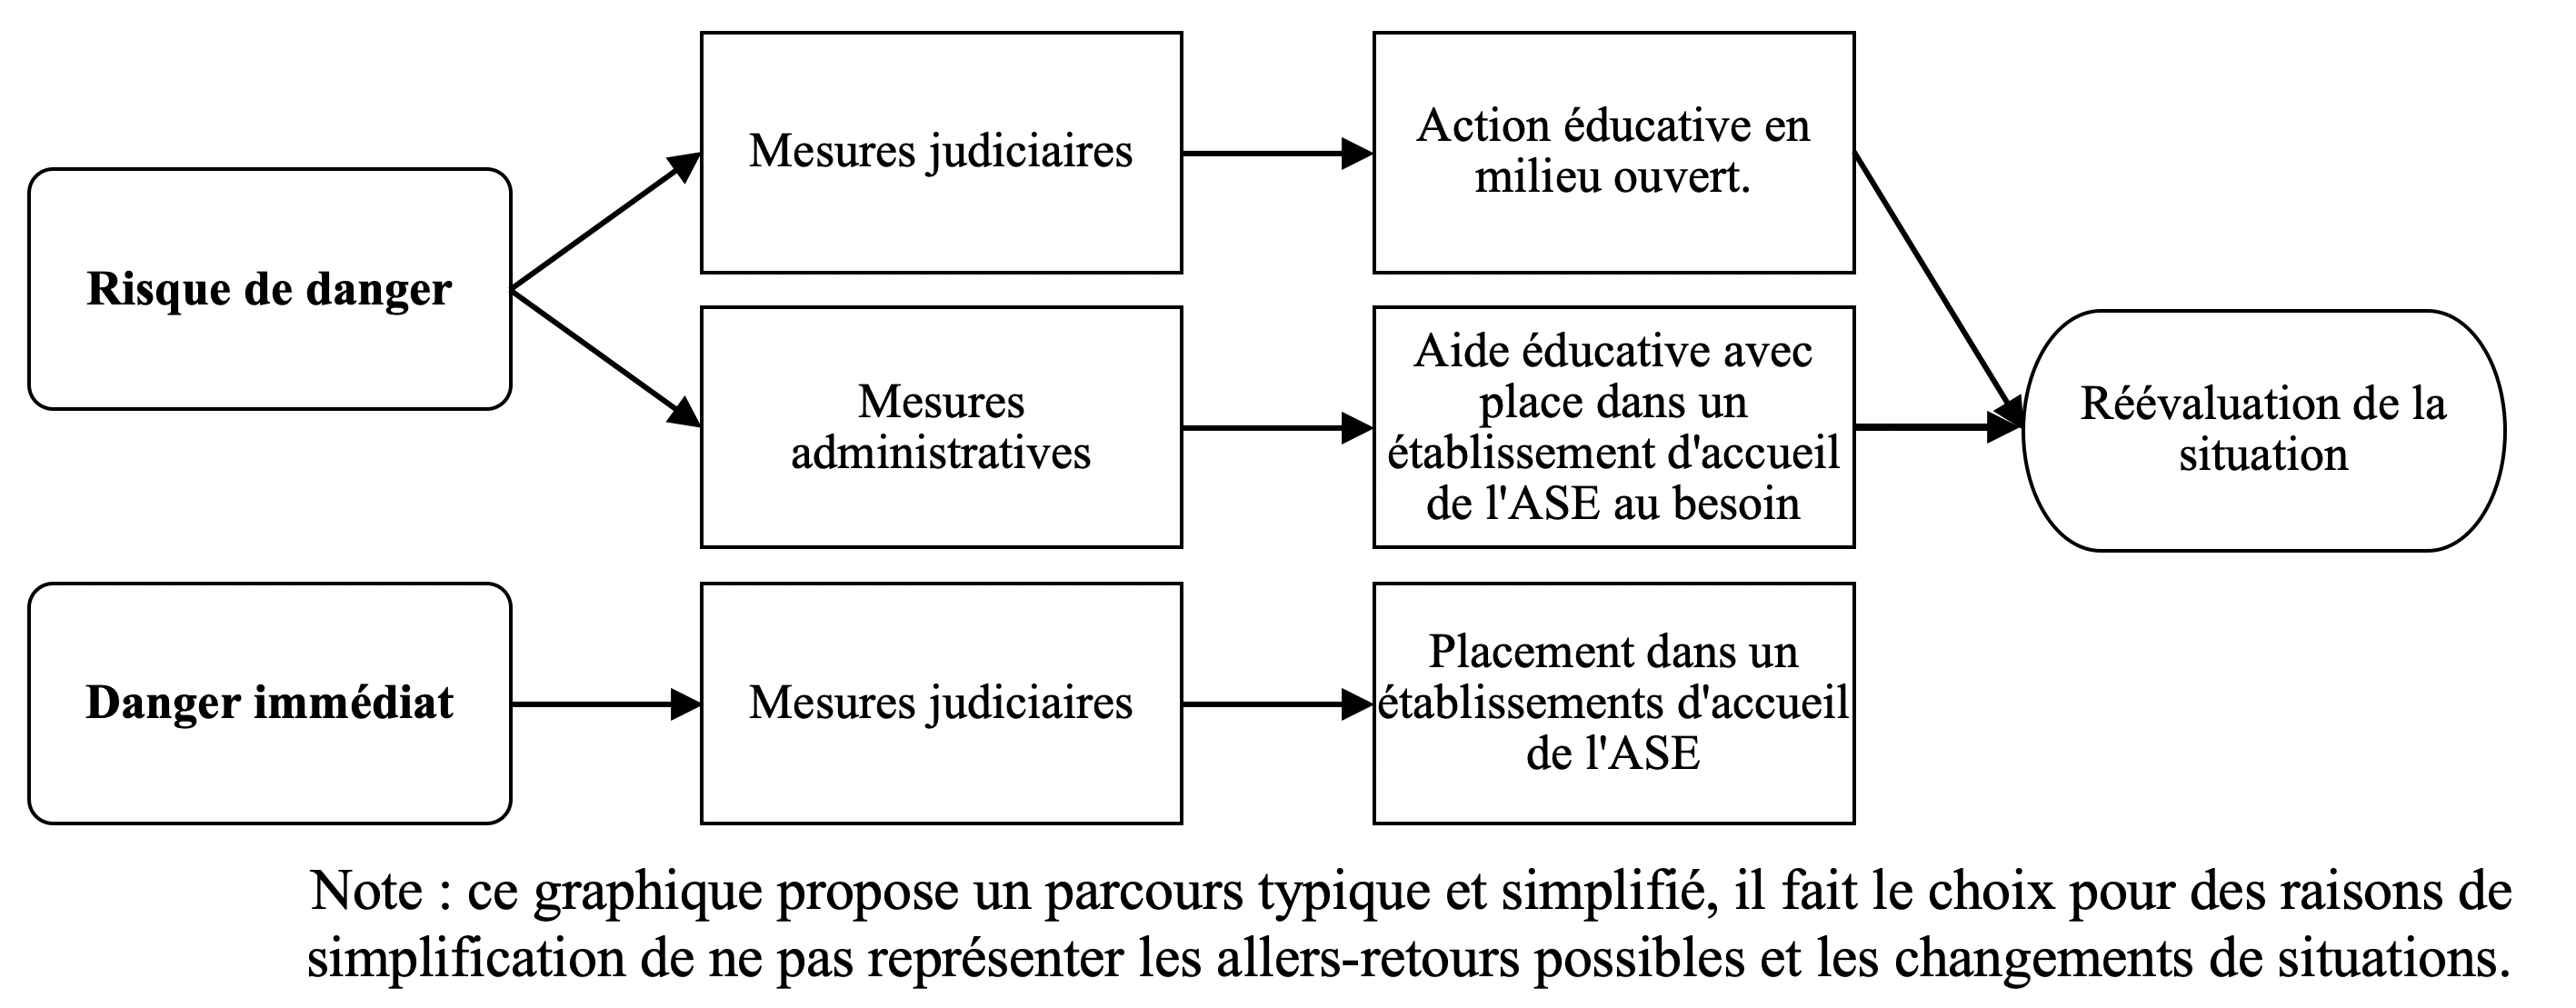
\includegraphics[width=0.8\linewidth]{Figure/SC2} \end{center}

\small\{Note : ce graphique propose un parcours typique et simplifié, il
fait le choix pour des raisons de simplification de ne pas représenter
les allers-retours possibles et les changements de situations.\}

Ainsi, après signalement, la Cellule de recueil des informations
préoccupantes (Crip) enquête sur la situation de l'enfant. Cette
première étape consiste à une visite d'une assistante sociale au
domicile de l'enfant, elle tente alors de déterminer s'il y a risque de
danger ou danger immédiat. Mais aussi, elle cherche à savoir si les
parents sont enclins à accepter une aide. Suite à cette visite,
l'assistante sociale fait remonter en cas de risque de danger ou danger
immédiat l'information, afin qu'une aide soit mise en place.

S'il y a selon elle danger immédiat, l'affaire est envoyée au juge des
enfants qui jauge la situation et tente de mettre en place une mesure de
commun accord avec les parents ou tuteurs légaux. Dans le cas du danger
immédiat, c'est néanmoins le juge des enfants qui a le dernier mot en la
matière, il n'a donc pas besoin de recueillir l'aval des parents ou
tuteurs légaux. Une mesure judiciaire va être prise qui débouche sur un
placement en famille d'accueil, Maison d'enfant à caractère sociale,
pouponnières ou villages d'enfants.

S'il y a risque de danger, une assistance éducative va être proposée par
le département et être appliquée généralement sous la forme d'une aide
éducative à domicile si les parents sont d'accord. Si les parents
refusent ou que l'aide éducative à domicile échoue, l'affaire peut être
transférée au juge des enfants qui peut dès lors prendre une mesure sans
l'aval des parents. Généralement, une mesure d'action éducative en
milieu ouvert, couramment appelée AEMO, est mise en place. La situation
de l'enfant est à la fin réévaluée. Si le risque de danger persiste ou
que l'AEMO est un échec, l'affaire est renvoyée devant le juge des
enfants qui reconduit la mesure ou décide d'un placement.

Le processus de placement suit ainsi un parcours type qu'émilie Potin
s'est attachée à décrire d'un point de vue sociologique prenant en
compte l'expérience de l'enfant. Elle décrit ainsi le parcours de
placement comme traversé par trois phases principales : « la désignation
du danger (processus d'étiquetage) », puis le « déplacement d'un lieu à
l'autre et d'un milieu social à l'autre (processus d'apprentissage,
d'adaptation et de socialisation) » et enfin : « l'intégration dans le
quotidien du placement (phase de routinisation) » . Le processus
d'étiquetage appelle par la suite à un déplacement dans une structure. à
l'aide de l'étiquette attribuée à la situation de l'enfant, l'ASE
appelle ensuite les structures qu'elle juge adaptées à accueillir
l'enfant afin d'appliquer la décision de protection. Les structures
elles-mêmes acceptent ou non d'accueillir l'enfant en fonction de leur
jugement en leur capacité d'accueillir l'enfant, leurs places
disponibles et le public déjà accueilli.

~~~\emph{Les catégories juridiques des enfants accueillis}

De ce système de protection résulte sept catégories juridiques d'enfants
protégés répartis en deux catégories : les mesures judiciaires et les
mesures administratives. Le tableau ci-dessous les présente.

Il est à noter que quand bien même un enfant entre à la Protection de
l'enfance dans une catégorie juridique, cette dernière n'est pas
immuable. Il peut ainsi, au moment de la réévaluation de sa situation,
se retrouver dans une autre catégorie pour pouvoir poursuivre sa prise
en charge à la Protection de l'enfance dans les meilleures conditions.
Pour la recherche scientifique, ces catégories juridiques font l'objet
de réflexion, puisqu'on les retrouve dans les données produites sur le
sujet. Ainsi, la question de leur utilisation et de leur signification
sociologique se pose comme le souligne I. Frechon . Le problème majeur
de ces catégories est qu'elles concentrent des enfants aux situations
très diverses dans les mêmes groupes. Ce point rend difficile de se
servir de ces catégories pour définir les enfants pris en charge,
néanmoins il rend utile de tels variables afin de porter son regard sur
les pratiques des professionnels et surtout les différences entre
pratiques du secteur judiciaire et du secteur administratif.

~~~~~~\emph{Définitions des différents types d'établissements et
d'hébergements}

Nous venons brièvement de l'évoquer dans le parcours type de placement,
mais il existe différents lieux d'accueil qui sont destinés à accueillir
les enfants en fonction de leurs besoins individuels, c'est-à-dire en
fonction de leur âge, de leur motif de placement et d'éventuelles
particularités dans leur situation : mineurs non accompagnés, situation
de handicap.

Si on structure ce tour d'horizon des types d'établissements de
placement de l'ASE par âge, il convient de débuter avec les
pouponnières. Ces dernières sont spécialisées dans l'accueil des tout
petits enfants de 0 à 3 ans, ce sont des structures de taille moyenne
avec comme capacité autorisée en 2017 une moyenne de 23 places,
n'excédant pas les 30 places dans 75\% des cas en 2017.

Ensuite, les villages d'enfants sont peu nombreux sur le territoire, 37
structures en tout. Ils sont spécialisés dans l'accueil des enfants sur
le long terme. Ce sont de grandes structures avec une capacité moyenne
de 57 enfants par structures répartis en unité de vie, ce qui permet de
proposer néanmoins un accueil personnalisé et une stabilité dans le
placement.

Les lieux de vie et d'accueil proposent quant à eux un accueil
individualisé des enfants dans de petites structures ayant en moyenne 6
places et qui ne peuvent accueillir plus de 7 enfants. Ils accueillent
les enfants avec des problèmes psychologiques ou ceux que l'on considère
comme des « incasables », c'est-à-dire qui enchainent les types de
placement, sans qu'aucun ne semble parvenir à s'adapter à leurs besoins.

Les Foyers de l'enfance sont des hébergements d'urgence et courts qui
accueillent surtout avant réorientation les enfants vers un type
d'accueil plus pérennes. Ce sont des structures de taille variable avec
une capacité moyenne de 58 enfants. 25\% de ses structures ne dépassent
pas les 12 enfants en capacité d'accueil autorisée et 25\% dépassent à
l'inverse les 63 enfants en capacité d'accueil autorisée.

Enfin, les Maisons d'enfant à caractère social (MECS), propose un
accueil temporaire d'enfant lié à un problème familial ou
comportemental. Ils accueillent aussi les mineurs non accompagnés. Ils
ont une capacité moyenne d'accueil de 41 enfants avec aussi une grande
variabilité en 2017 dans la taille des structures : un premier quart de
structures ne dépassant pas 18 places en capacité autorisée, la moitié
les 35 et enfin les trois-quarts les 56.

Le premier type d'hébergement le plus courant et proposant le plus de
places est l'internat collectif. C'est un hébergement au sein de la
structure qui peut proposer plusieurs unités de vie, c'est le cas
notamment dans les villages d'enfant. On le retrouve dans tous les types
d'établissements.

Le deuxième type d'hébergement sont les assistants familiaux. Ces
derniers sont des professionnels de la protection de l'enfance formés
par l'état à l'accueil de mineurs ou jeunes majeurs protégés. Ils
accueillent directement chez eux les jeunes majeurs ou mineurs. Ils
restent rattachés dans certains cas à des établissements qui gèrent le
placement de l'enfant et on les retrouve aussi dans tous les types
d'établissements.

Le placement à domicile est une mesure d'assistance éducative décidée
par un juge pour enfant. Concrètement, le jeune majeur ou le mineur
continue de vivre dans sa famille, mais bénéficie d'une solution de
repli dans un établissement de l'ASE. C'est un type d'hébergement que
l'on retrouve dans tous les types d'établissements, sauf en lieux de vie
et d'accueil.

Enfin, le logement autonome ou hébergement éclaté recoupe plusieurs
réalités. Il s'agit de place d'hébergement physiquement en dehors de la
structure d'accueil, soit dans un ensemble de logements, soit en
chambres dispersées dans le logement ordinaire ou l'habitat social,
voire en hôtel. C'est un type d'hébergement qui n'est logiquement pas
proposé par les pouponnières à caractère social et est peu présent dans
les villages pour enfants.

\hypertarget{limpossible-comptabilisation-des-enfants-placuxe9s-un-enjeu-de-gestion-et-de-recherche}{%
\section{L'impossible comptabilisation des enfants placés ? Un enjeu de
gestion et de
recherche}\label{limpossible-comptabilisation-des-enfants-placuxe9s-un-enjeu-de-gestion-et-de-recherche}}

\hypertarget{les-effets-de-la-duxe9partementalisation-sur-la-production-de-donnuxe9es}{%
\subsection{Les effets de la départementalisation sur la production de
données}\label{les-effets-de-la-duxe9partementalisation-sur-la-production-de-donnuxe9es}}

~~~~~~\emph{Une organisation héritée de la décentralisation}

Les lois de décentralisation de 1983 et 1984 ont transféré la compétence
\textless\textless{} d'aide aux enfants confrontés à des difficultés
sociales susceptibles de compromettre gravement leur équilibre
\textgreater\textgreater{} (CASF, Article L221-1) aux présidents des
Conseils généraux et ont précisé les contours de l'autorité judiciaire
et de l'autorité administrative. Dès lors, la branche judiciaire
intervient dans le cas où les mineurs victime de mauvais traitements
voit leur famille refuser l'intervention du service de l'Aide sociale à
l'enfance. Le président du Conseil Général voit ses missions en la
matière précisées : il définit la politique départementale de l'aide
sociale à l'enfance, crée et autorise les établissements sociaux et
arrête leur tarification, et enfin, il prononce l'admission à toute
mesure d'aide sociale à l'enfance .

Cette décentralisation a eu des effets concrets sur la production de
statistiques sur le sujet. En effet, historiquement les statistiques
sont liées à l'état et particulièrement à l'état-providence qui au cours
du XXe siècle s'est aidé de ces outils permettant d'estimer la capacité
et les besoins d'une population pour bâtir ses politiques sociales et
les piloter à long terme. Pour A. Desrosières, le modèle français serait
un mélange d'une tradition administrative centralisée et d'un
rationalisme, en témoigne l'exemple des ingénieurs administrateurs . à
contre-courant de cela, la décentralisation de l'aide sociale a rendu
particulièrement difficile la production de statistiques globale sur la
Protection de l'enfance, en plus de créer des disparités départementales
en matière de politique de l'aide sociale. Cette situation a créé de
l'ignorance qui a des conséquences autant gestionnaires et politiques
que sur l'état de la recherche scientifique sur ces sujets.

Pourtant, la visée statistique était bien présente dans la loi de 1989
qui prévoyait la remontée de données en chargeant les présidents du
Conseil Général de mettre en place un dispositif de recueil
d'informations. Dès 1991, une première étude de faisabilité réalisée par
l'Institut de l'enfance et de la famille dresse l'état des lieux de la
collecte statistiques sur le sujet en France et ébauche un dispositif de
recueil. Pourtant, il faut attendre 1997 avec l'Observatoire national de
l'action sociale décentralisée (ODAS) pour qu'une méthodologie
d'observation à l'échelle nationale soit élaborée avec le concours des
départements. C'est ainsi qu'est née le recensement annuel des
signalements transmis aux département, premier jalon d'une statistique
nationale sur le sujet, malgré l'existence de données produites par la
DREES qui ne s'intéresse elle depuis 1982 qu'aux établissements sociaux.
Cette enquête de la DREES n'était pas dédiée à la Protection de
l'enfance puisqu'elle portait alors autant sur les établissements et
services pour personnes handicapées que sur ceux pour personnes en
difficulté sociale, et donc de la Protection de l'enfance.

~~~~~~\emph{La création de la ONPE}

Dès lors, dans les années 2000, l'état cherche à organiser des
structures à l'échelle nationale à même de produire des connaissances
sur la Protection de l'enfance et de rationnaliser la collecte de
données. L'observatoire national de la Protection de l'enfance (ONPE)
est créé dans cette optique en 2004. Les lois de 2004 et 2007 établies
ses principales missions qui sont les suivantes : « Améliorer la
connaissance sur les questions de mise en danger et de protection des
mineurs à travers le recensement et le développement des données
chiffrées d'une part, des études et recherches d'autre part ; Recenser,
analyser et diffuser les pratiques de prévention et d'intervention en
protection de l'enfance ; Soutenir les acteurs de la protection de
l'enfance. » (CASF, art L 226-6). Avec la loi du 7 février 2022, la
définition de son rôle est renforcée et il devient un « centre national
de ressource, chargé de recenser les bonnes pratiques et de répertorier
ou de concourir à l'élaboration d'outils et de référentiels » (CASF, art
L 226-6).

Sa production principale est depuis sa création l'estimation annuelle du
nombre d'enfants protégés. Ce chiffre est le résultat du croisement des
données de deux principales sources : de la Direction de la recherche,
des études, de l'évaluation et des statistiques (DREES) et de la
Direction de la protection judiciaire de la jeunesse (DPJJ). Ainsi, en
2015, le nombre de mineurs bénéficiant d'au moins une mesure de
protection de l'enfance est estimé à 295 357 sur la France entière, soit
20,1 ‰ des moins de 18 ans .

~~~~~~\emph{Les observatoires départementaux}

En appui de l'ONPE, la loi de 2007 cherche à compléter le dispositif de
remontée des données départementales sur la Protection de l'enfance en
créant des observatoires départementaux de la protection de l'enfance
(ODPE). C'est le président du Conseil Général qui est chargé de leur
mise en place et de leur animation en association avec les acteurs
locaux. Pourtant la mise en place de ces observatoires et leur
effectivité a fait l'objet de nombreuses difficultés, tant et si bien
qu'encore en 2020, l'ONPE continue de produire des documents dressant
des états des lieux de la mise en place des ODPE sur le territoire. En
effet, l'ONPE suit attentivement depuis 2009 le développement de ces
observatoires à l'aide d'une enquête bisannuelle qui les interroge sur
leur fonctionnement autant que sur leurs attentes, besoins et
difficultés. En 2020, 83 observatoires départementaux sont installés et
10 sont en construction, sur les 100 départements existants en France
métropolitaine et DROM, hors Mayotte. 4 départements font encore figure
d'exception en n'ayant pas prévu la construction d'ODPE. En 2018, 17
ODPE étaient construction et 74 déjà en place. L'absence d'ODPE ne
signifie pas pour autant absence de production de statistiques sur le
sujet. En effet, sur 14 départements encore non-dotés d'observatoire, 11
d'entre eux ont tout de même mis en place un dispositif ou des instances
permettant de recueillir des données quantitatives et/ou qualitatives.

Les ODPE font face aujourd'hui à des difficultés d'ordre technique et
réclament autant des formations qu'un soutien technique de la part de
l'ONPE pour les aider dans la gestion et la production de données . Les
départements apparaissent ainsi en demande de soutien pour bâtir des
systèmes de collecte statistiques efficaces leur permettant de mieux
connaître la portée sur leur territoire de leur politique départementale
d'aide sociale. Ainsi, la mise en place de structures adaptées semble
difficile au niveau départemental pour ces raisons, mais aussi parce
qu'ils rencontrent des obstacles au niveau local des structures
d'accueil. En effet, ces dernières sont logiquement chargées de
communiquer des informations sur le public accueilli et les places
disponibles, mais cette remontée est rendue difficile d'une part du fait
d'un manque de formation du personnel en charge de remplir ces bases et
d'autre part du fait d'une crainte que l'utilisation de ces données ne
mène à une baisse de la subvention de ces lieux d'accueil. Ces
difficultés concernent dès lors autant les enquêtes menées par l'ONPE,
que celles menées par la DREES qui s'adresse directement aux structures
d'accueil.

\mdfsetup{%
middlelinewidth=2pt,
backgroundcolor=gray!10,
roundcorner=10pt}
\begin{mdframed}[frametitle= Exemple d'une rencontre avec un chargé de mission de la direction enfance et famille et de l'ODPE du département de l'Hérault]

Cette rencontre réalisée dans le cadre d'une discussion sur un projet de thèse en contrat CIFRE exemplifie certaines difficultés dans la production de données rencontrées par les départements, pourtant envieux d'approfondir leurs connaissances sur leurs dispositifs d'aide sociale à l'enfance. Ainsi, à la fin de l'année 2021, le projet de recherche que le département de l'Hérault souhaitait financer visait, à l'aide des données qu'ils produisent, à chercher à « prendre du recul » sur les effets de leurs politiques départementales. à titre indicatif, selon le chargé d'études et directeur de l'ODPE de l'Hérault, la direction enfance et famille traite 2500 informations préoccupantes, suit 2700 enfants à domicile dans leurs familles et accueille près de 2800 enfants et jeunes majeurs en foyers et en famille d'accueil en 2021.

Il témoigne de leur besoin de visibilité sur leurs disponibilités d'accueil, les contours de leur accueil familial et sur les usages des dispositifs. En particulier, ils ont besoin qu'un travail soit mené sur les mesures administratives et judiciaires et leurs différentes déclinaisons. Mais aussi sur les mesures de préventions, puisqu'actuellement ils peinent à avoir des données qui leur permettent de justifier de l'intérêt des politiques de prévention sur celles d'accueil. Ce sont des questions certes techniques, mais qui cachent aussi des enjeux financiers importants pour le département.

Au niveau de leur données, comme de nombreux autres départements, ils utilisent un logiciel qui leur permet de faire des extractions suivant des requêtes, mais leur base de données dispose de peu d'informations sur le profil socio-économique de l'enfant accueilli et de sa famille. Ce point rend l'analyse sociologique difficile. Le département chercherait ainsi à améliorer leur base de données, afin de la rendre effective pour qu'elle réponde aux questions de politiques public qu'ils se posent. Cette recherche se serait faite avec les données regroupées suite à une compilation manuelle de l'ODPE de l'Hérault. Cette dernière est une instance partenariale regroupant le Département de l'Hérault, des MECS (Maisons d'enfant à caractère social) et lieux de vie, des assistants familiaux, l'éducation nationale, l'école des travailleurs sociaux et des associations œuvrant pour la protection de l'enfance. Elle a été créée récemment puisque leur première séance plénière s'est tenue en 2019. Cette remontée des données prend appui sur des assistantes administratives qui remplissent les bases, ce qui peut donner lieu à des erreurs du fait qu'il ne s'agit pas d'un personnel formé pour accomplir cette tâche. Ce point allié à d'autres difficultés techniques fait qu'à l'heure actuelle le département lui-même a du mal à dire où il y a des places disponibles dans les lieux d'accueil et d'hébergement. Le chargé de mission et directeur de l'ODPE de l'Hérault suppose ainsi que l'orientation des enfants dans tel ou tel type d'hébergement dépend essentiellement de l'offre et de la demande.

\end{mdframed}

\newpage
\singlespacing
\setlength{\parskip}{0.5em}

\phantomsection
\addcontentsline{toc}{section}{Bibliographie}
\section*{Bibliographie}

\hypertarget{refs}{}
\begin{CSLReferences}{0}{0}
\end{CSLReferences}

\end{document}
